% Options for packages loaded elsewhere
\PassOptionsToPackage{unicode}{hyperref}
\PassOptionsToPackage{hyphens}{url}
%
\documentclass[
]{article}
\usepackage{amsmath,amssymb}
\usepackage{lmodern}
\usepackage{ifxetex,ifluatex}
\ifnum 0\ifxetex 1\fi\ifluatex 1\fi=0 % if pdftex
  \usepackage[T1]{fontenc}
  \usepackage[utf8]{inputenc}
  \usepackage{textcomp} % provide euro and other symbols
\else % if luatex or xetex
  \usepackage{unicode-math}
  \defaultfontfeatures{Scale=MatchLowercase}
  \defaultfontfeatures[\rmfamily]{Ligatures=TeX,Scale=1}
\fi
% Use upquote if available, for straight quotes in verbatim environments
\IfFileExists{upquote.sty}{\usepackage{upquote}}{}
\IfFileExists{microtype.sty}{% use microtype if available
  \usepackage[]{microtype}
  \UseMicrotypeSet[protrusion]{basicmath} % disable protrusion for tt fonts
}{}
\makeatletter
\@ifundefined{KOMAClassName}{% if non-KOMA class
  \IfFileExists{parskip.sty}{%
    \usepackage{parskip}
  }{% else
    \setlength{\parindent}{0pt}
    \setlength{\parskip}{6pt plus 2pt minus 1pt}}
}{% if KOMA class
  \KOMAoptions{parskip=half}}
\makeatother
\usepackage{xcolor}
\IfFileExists{xurl.sty}{\usepackage{xurl}}{} % add URL line breaks if available
\IfFileExists{bookmark.sty}{\usepackage{bookmark}}{\usepackage{hyperref}}
\hypersetup{
  pdftitle={MTBrush\_paper},
  pdfauthor={Yixing Tu},
  hidelinks,
  pdfcreator={LaTeX via pandoc}}
\urlstyle{same} % disable monospaced font for URLs
\usepackage[margin=1in]{geometry}
\usepackage{graphicx}
\makeatletter
\def\maxwidth{\ifdim\Gin@nat@width>\linewidth\linewidth\else\Gin@nat@width\fi}
\def\maxheight{\ifdim\Gin@nat@height>\textheight\textheight\else\Gin@nat@height\fi}
\makeatother
% Scale images if necessary, so that they will not overflow the page
% margins by default, and it is still possible to overwrite the defaults
% using explicit options in \includegraphics[width, height, ...]{}
\setkeys{Gin}{width=\maxwidth,height=\maxheight,keepaspectratio}
% Set default figure placement to htbp
\makeatletter
\def\fps@figure{htbp}
\makeatother
\setlength{\emergencystretch}{3em} % prevent overfull lines
\providecommand{\tightlist}{%
  \setlength{\itemsep}{0pt}\setlength{\parskip}{0pt}}
\setcounter{secnumdepth}{-\maxdimen} % remove section numbering
\ifluatex
  \usepackage{selnolig}  % disable illegal ligatures
\fi

\title{MTBrush\_paper}
\author{Yixing Tu}
\date{3/25/2022}

\begin{document}
\maketitle

\hypertarget{abstract}{%
\section{Abstract}\label{abstract}}

To analysis data made of n group of m measurements and p parameters
especially when n is large, one approach is fitting a set of models for
each group and getting the n test statistics. Since the number of group
is large, it is not easy to compare among groups and extract marginal
cases directly from test statistics. Visualization can make extreme
cases stand out from the population. MTBrush is an R package that can be
used to conduct and visualizing such multiple hypothesis tests for such
high dimensional datasets. It allows users to fit n regression models
and visualizing histograms of test statistics. To further investigate
results, it adds an interactive tools allowing users to brush through
histograms and query for significant groups. By comparing the
highlighted part in the histograms of different terms and with the help
of corresponding scatter plots, users can easily identify whether the
interaction terms have synergistic or competitive effects and then make
informative conclusions.

\hypertarget{keywords}{%
\section{Keywords}\label{keywords}}

Multiple hypothesis testing, interaction diagrams, R package;

\hypertarget{introduction}{%
\section{Introduction}\label{introduction}}

When dealing with high volume dataset such as taking repetitive
measurements over many samples with slight change on one parameter each
time especially in microbiome and microarray study, a large amount of
test statistics will be generated by performing large-scale testing. For
example, according to Efron and Hastie in the book ``Computer Age
Statistical Inference'', to make analysis for the prostate cancer data
which contained n = 102 samples, 52 experimental samples and 50 controls
and N = 6033 genes and 6033 * 102 matrix of measurements. In this study,
a two-sample t statistics was applied to each gene, and generated 6033
test statistics in total. When more than one parameters are measured,
the two-sample t statistics is not applicable, then we can fit a
collection of regression models, one per sample. It will be easier to
compare when all statistics come from the same model. We use this
fitting models approach in our package to set up the hypothesis testing
and interpreted the effects from the test results.

After having the test statistics, it can be tedious and time consuming
to analyze results from the multiple hypothesis testing procedure due to
the large amount. Visualization of statistics can help to reveal some
information from the data. A common approach is generating histograms of
test statistics to compare with the null threshold curve and distinguish
the non-null cases on the tails. Using the same example as above, they
drew a histogram for 6033 t statistics and compared the distribution
with the scaled N(0,1) density curve, all genes under the curve were
consider as null. With this histogram, one can notice that there are
some non-null genes around the tails, but there is no way to know the
gene id and measurements of those non-null genes and it is impossible to
pick out those genes and compare those with null genes. Therefore, one
were not able to tell the difference between null and non-null genes and
it is hard to tell whether the boundary cases were test error or
non-null indeed. It reveals the problem of this approach that histograms
can only tell the presence of significant cases, but it failed to locate
such cases so it prevent us from further interpreting the significance
in the data and giving examples to support our hypothesis about the
terms' effects. Also, it is especially hard to interpret plots as plots
getting complex in some high dimensional and multivariate studies
(Wills, 08). In the prostate data study, one gene of a man only has one
measurement, the situation will be more intricacy when there are
multiple measurements for each gene.

Those two problems can be solved by linking plots. Not trying to make a
complex plots explain everything from the data and test results, we
could build several simpler parts and link them together to help to
analyze the data. We decide to link test statistics with the information
form the raw data. We found that brushing has been used for connected
statistics on multiple levels to one another (Wickham), but there isn't
one for models under multiple hypothesis settings. Therefore, this
package is trying build the linked visualizations for multiple
hypothesis testing studies. By brushing through one of the histogram,
samples in the brushed region will be selected. Selected samples will be
highlighted in all histograms so we can see the distribution of
statistics of other parameters for those samples. A table of all
parameters' test statistics of selected samples is present so we can
take a look at the average change in the presence of each parameter and
the extent of effects for the interaction terms. To link histograms of
test statistics with raw data, the scatter plots of selected sample with
measurements under each term will appear after brushing so we can check
if a large statistic accords with increase of measurement for some
samples. With the help of these functions, it will be much easier to do
analysis for large scale hypothesis testing.

For the rest of this paper, the methods part will discuss the basic
function, input, and output of each method in the the package and how to
use those methods to make multiple hypothesis testing analysis on a data
set. The case study will provide two examples under microbiome and house
prices context of applying this package to find the interaction effect
of different terms on each other. In the end, the discussion section
will talk about the future direction of this research.

\hypertarget{methods}{%
\section{Methods}\label{methods}}

\hypertarget{implementation}{%
\subsection{Implementation}\label{implementation}}

After load a data set, we first need to split samples into some groups
based on some criteria then we can apply hypothesis testing to each
group by fitting to parallel models chosen by users. Then with test
results, we will make one statistical histogram for one term to show the
distribution of this term's test statistics and those histograms will
serve as base plots of our shiny app. By brushing through any histogram,
all samples in the selected region and opposite side will be highlighted
in all histograms. At the same time, the scatter plots of selected
samples will appear to give information from the loading dataset and the
test statistics of those samples will be shown in a chart. With this
design, we could select extreme cases from a histogram and see the
distribution of those cases in other histogram to get some hints on if
the two measurements have positive or negative effects or no effect on
each other at all. For example, in the figure ``Interface after
brushing'', we brush on B term. If we look at the histogram of BK
interaction term, we found that the red points distributed on the left
side. It could be a hint that K has a negative effect on B. Then by
looking into details of test statistics and measurements of those
samples and compare those information with other samples, we could make
conclusions on possible correlations between variables and explain those
effects.

The package contains five methods:

\textbf{split\_dataset(df, group)}: This function splits the given data
set into many smaller subsets based on the group. Each subset only
contains measurements of a sample and all subsets take same
measurements.

\emph{parameters}:

df: the given data frame;\\
group: the name of the group column

\emph{return}: groups of subsets

\textbf{fit\_statistics(subsets, lm\_func, group)}: This method helps to
fit a model chosen by users for all groups of subset.

\emph{parameters}:

subsets: groups of subset from split\_dataset function;\\
lm\_func: the linear model chosen by user to fit the data;\\
group: the name of the group column

\emph{return}: a table with statistics of each term for all subsets

\textbf{draw\_stats\_histogram(stats\_df)}: This function provides a
part of the shiny app to generate several histograms of statistics for
each term

\emph{parameters}:

stats\_df: the output table from fit\_statistics function

\emph{return}: several histograms of all subsets based on terms in the
model

\textbf{brush\_plots\_binary(df, stats\_df, group\_list, group, value)}:
This method generates a shiny app displaying histograms of statistics
and scatter plots and a table of selected observations. Use this
function when the condition/explanatory variables have binary data type.

\emph{parameters}:

df: the processed data frame;\\
stats\_df: the output table from fit\_statistics function;\\
group\_list: a list of distinct observations;\\
group: the column name for grouping variable;\\
value: the column name for response variable;

\emph{return}: the shiny user interface contains histograms of
statistics and scatter plots and a table of selected observations.

\textbf{brush\_plots\_other(df, stats\_df, group\_list, group, value)}:
This method is similar to brush\_plots\_binary. It also generates a
shiny app displaying the histograms of statistics and scatter plots and
a table of selected observations. Use this function when the
condition/explanatory variables have non-binary data type.

\emph{parameters}:

df: the processed data frame;\\
stats\_df: the output table from fit\_statistics function;\\
group\_list: a list of distinct observations;\\
group: the column name for grouping variable;\\
value: the column name for response variable;

\emph{return}: the shiny user interface contains histograms of
statistics and scatter plots and a table of selected observations.

\begin{figure}
\centering
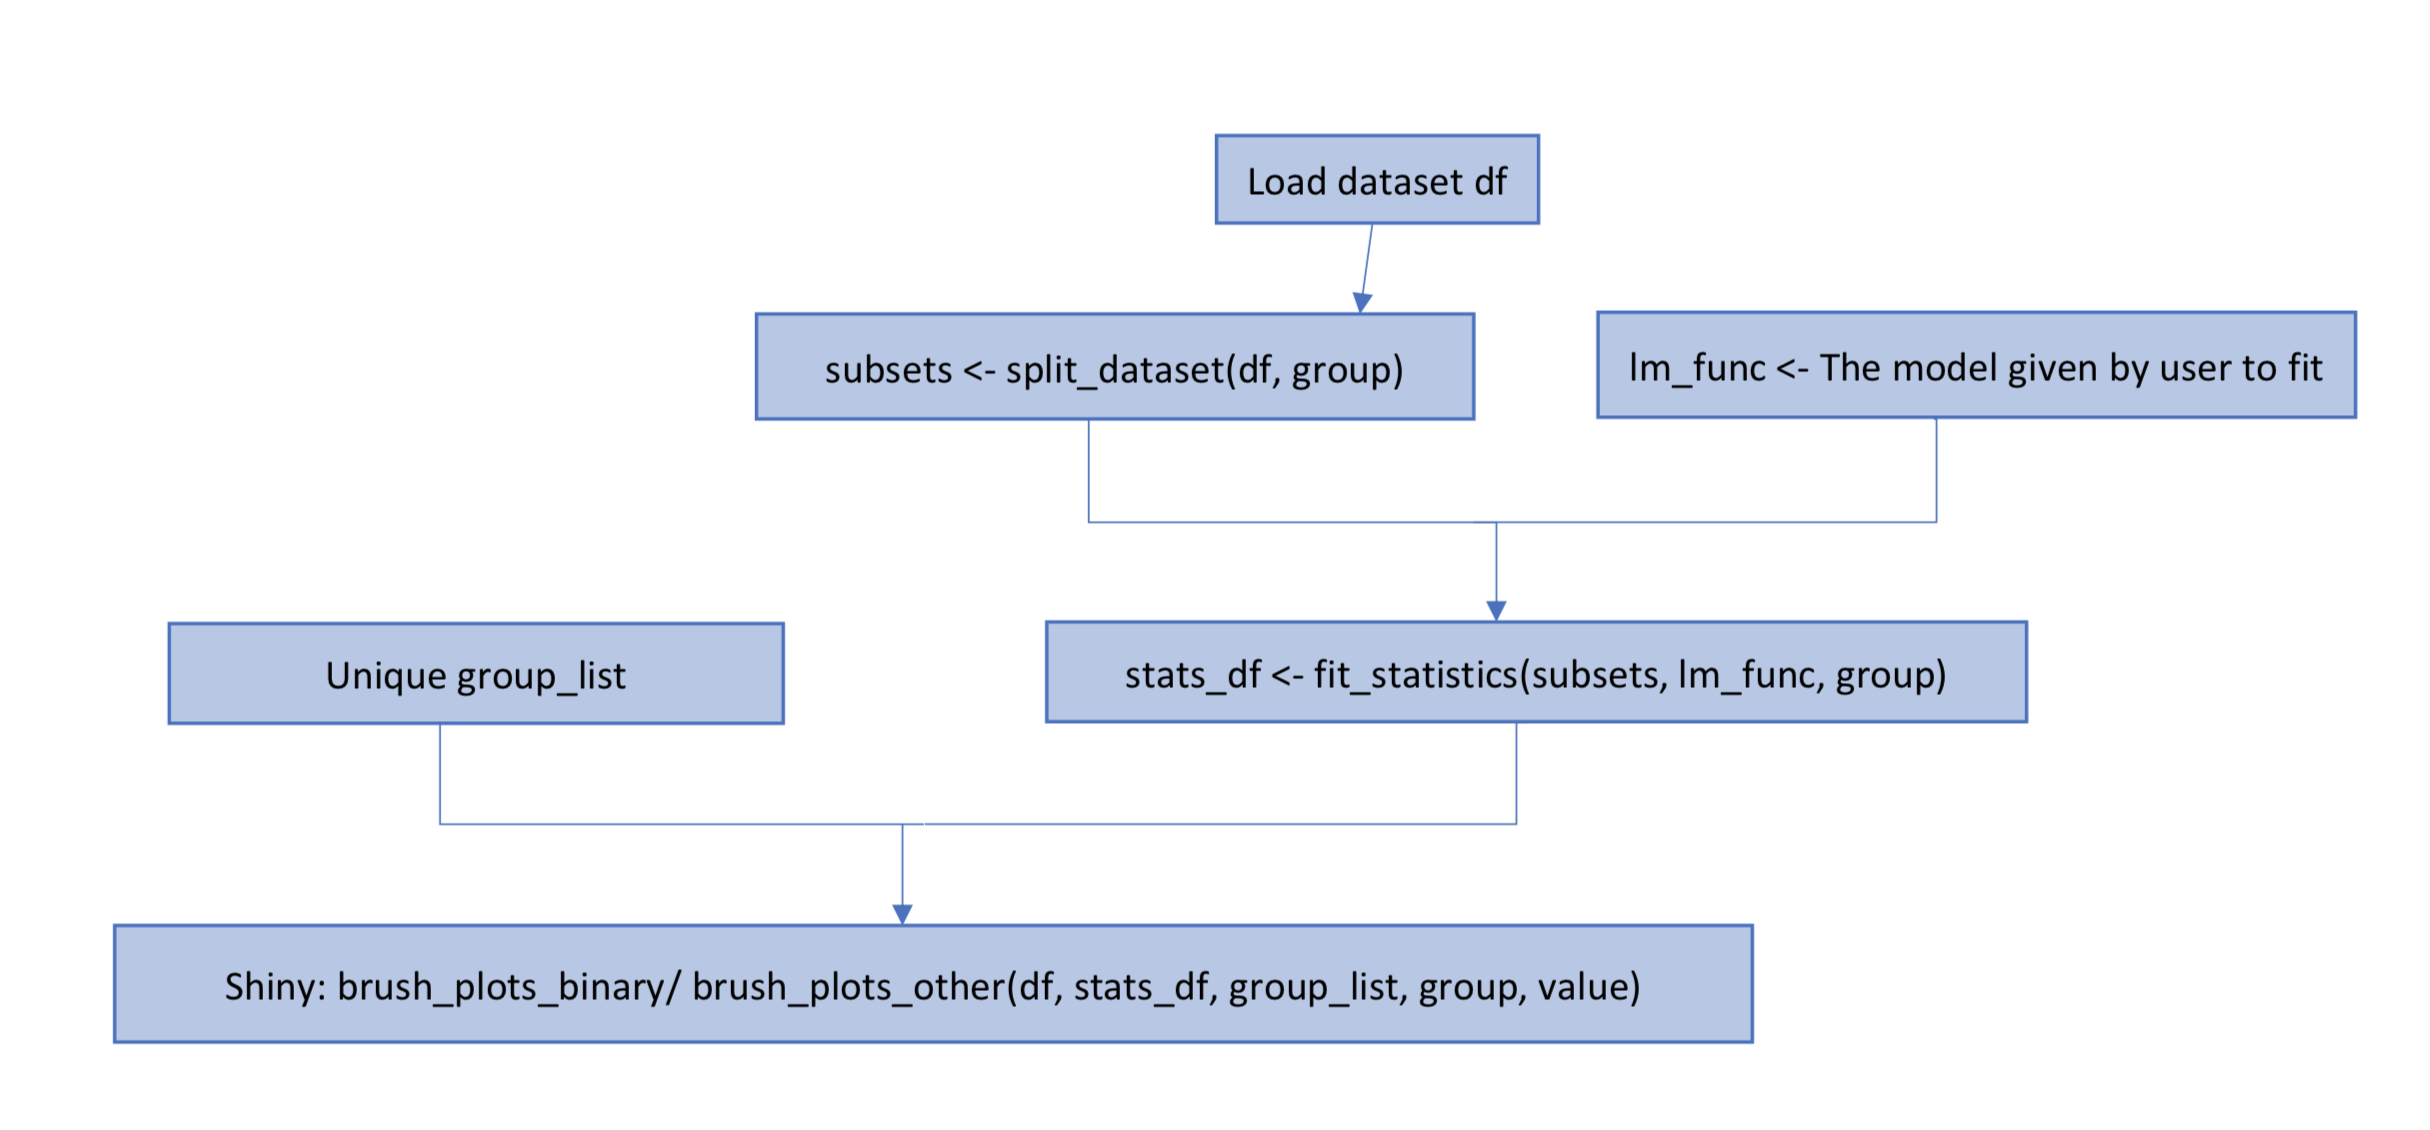
\includegraphics{/Users/tuyixing/Desktop/Course/research/workflow_pic.png}
\caption{Workflow}
\end{figure}

\hypertarget{operation}{%
\subsection{Operation}\label{operation}}

Before users make any interactions, the user interface of the generated
Shiny app is made of a group of histograms of statistics(section A) and
a scatter plot(section B) for all samples as shown in the figure
``Interface before interaction''. Users can brush through any histogram
on section A to query for significant samples on tails, then the
selected tail and the opposite end will be highlighted in different
colors as shown in ``Interface after brushing''. The scatter
plot(section D) will be replaced by a collection of scatter plots of
selected samples, which allow users to check details on each selected
samples. After brushing, a table(section F) will show up and the id of
selected samples are on section E and we can use the drop down menu in
this section to add or delete selected samples. From the table, Users
can also access the test statistics of each term for selected samples.
The test statistic value of the currently brushed histogram will
determine the order of compounds in the table. The most extreme value
will be at the top and the least extreme value will be at the bottom.
For example, if a user selects an interval on the B histogram, the first
compound in the table has the most extreme B test statistic. Also,
scatter plots are arranged in the same order as the table.

\begin{figure}
\centering
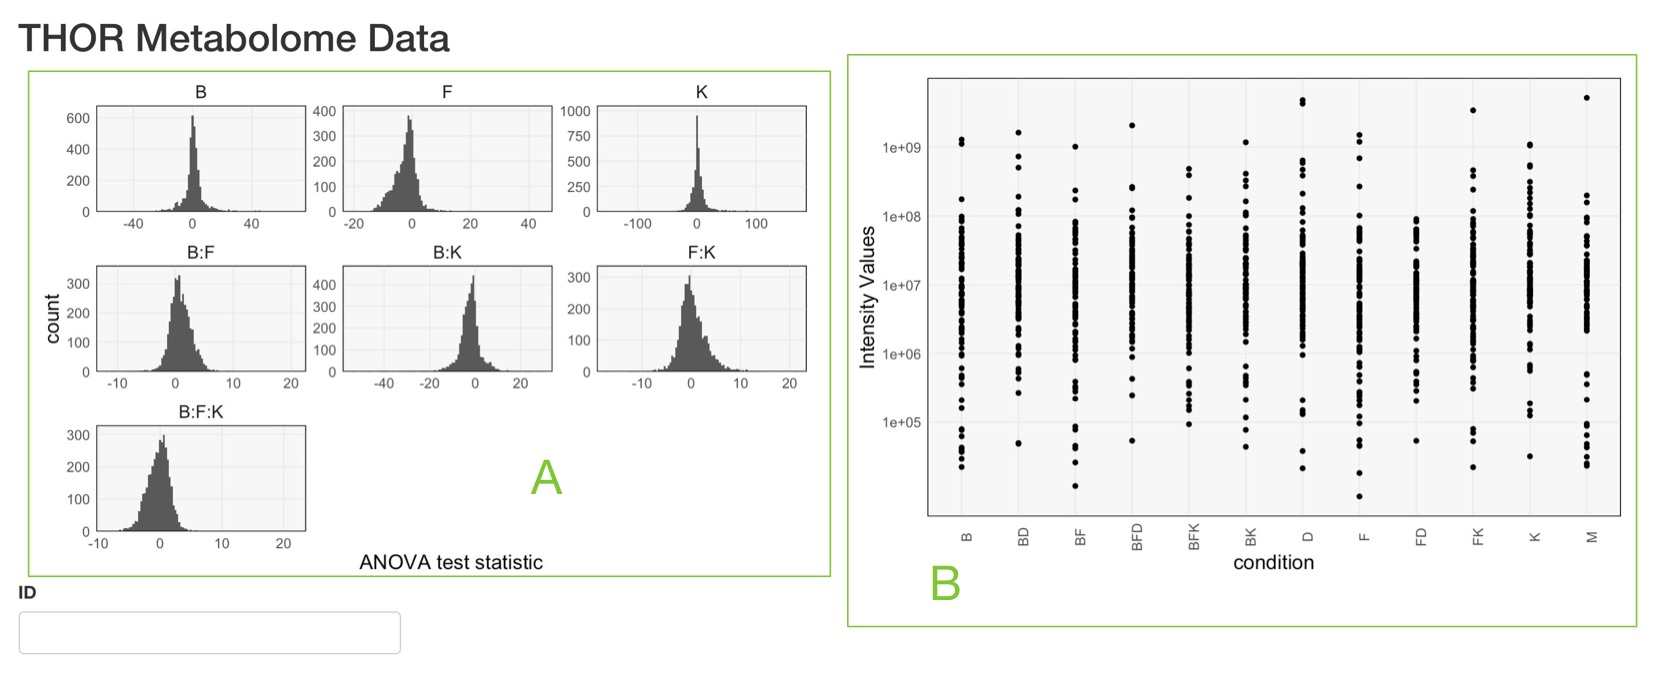
\includegraphics{/Users/tuyixing/Desktop/Course/research/interface1.jpg}
\caption{Interface before interaction}
\end{figure}

A: Histograms of test statistics, brush through any one of the histogram
to select samples;\\
B: Before brushing, a scatter plot of all samples will appear to give an
overall distribution of the dataset.

\begin{figure}
\centering
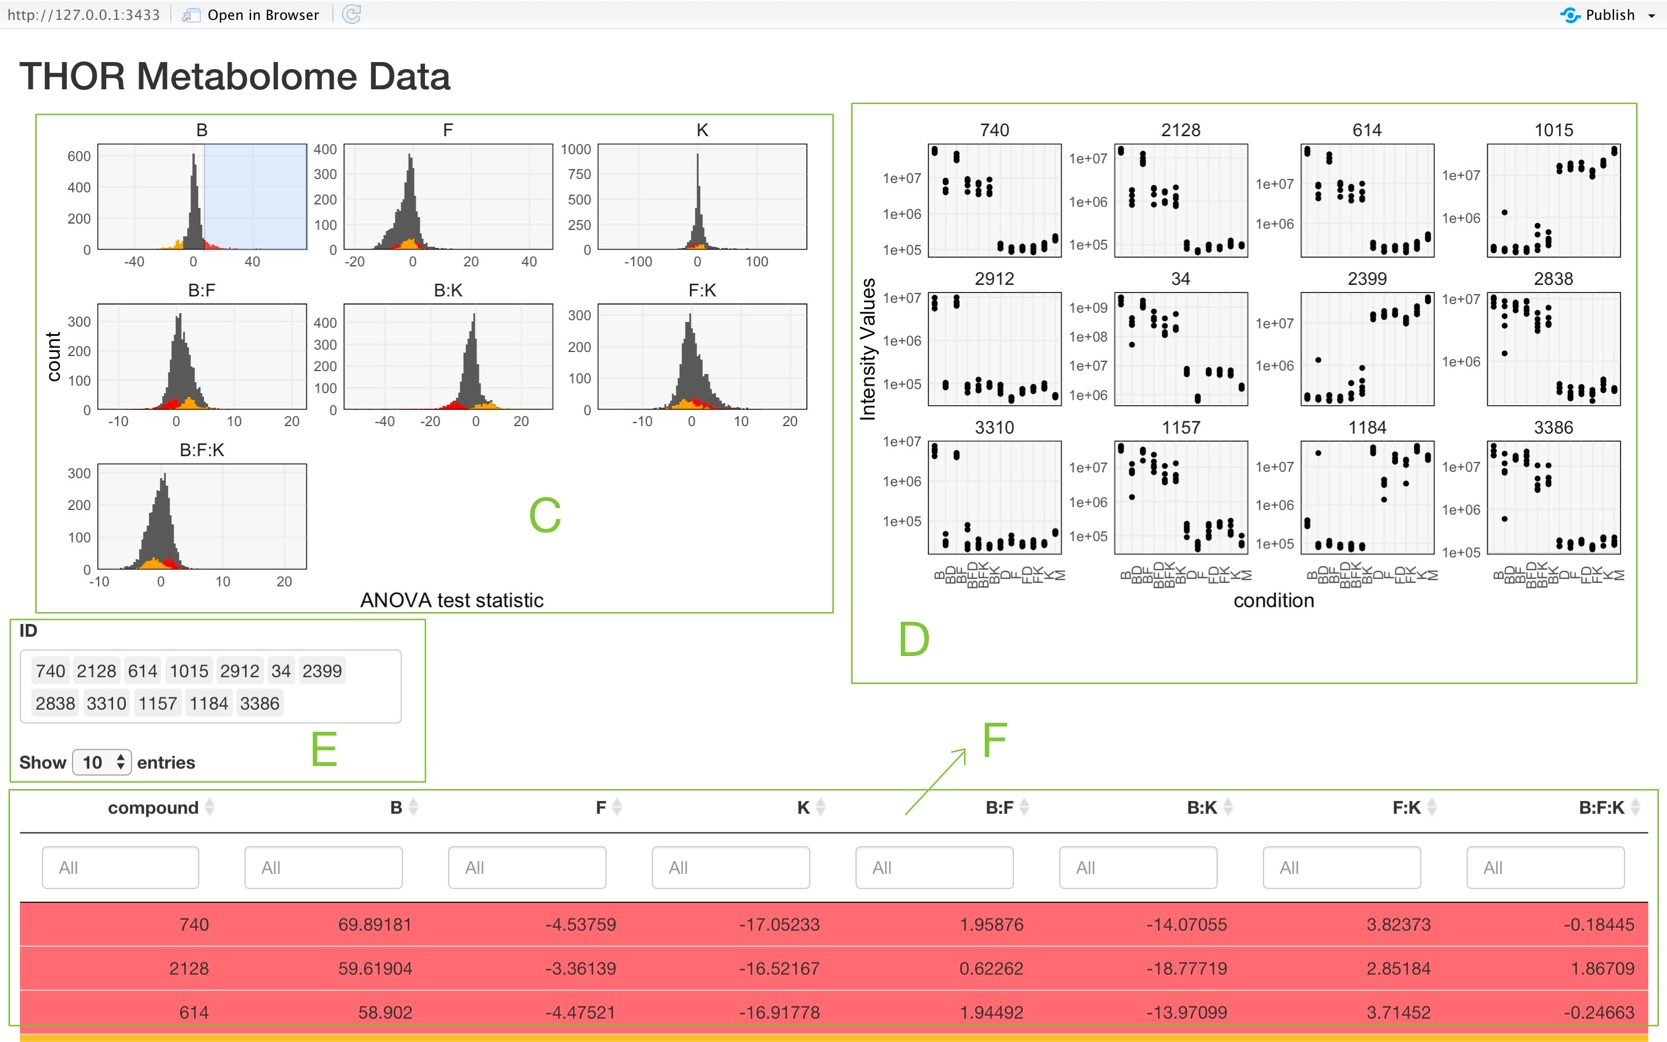
\includegraphics{/Users/tuyixing/Desktop/Course/research/interface2.jpg}
\caption{Interface after brushing}
\end{figure}

C: After brushing, test statistics greater than and less than the
threshold will be highlighted (red for positive and orange for negative
values). The selected samples will be highlighted in all histograms;\\
D: The scatter plots of top 12 samples in the table of selected samples
will be shown here. By adding or deleting the chosen ID on the left
select menu, users can choose to see the scatter plot of the sample they
have interests on;\\
E: By default, only 12 samples will be chosen at first. Users can use
the drop down menu to follow the samples of interests;\\
F: The table of selected samples in the brushed area. Color corresponds
to the color in the upper histograms.

\hypertarget{cases-studies}{%
\section{Cases Studies}\label{cases-studies}}

We illustrate the use of the \texttt{MTBrush} package using two case
studies. Our examples are drawn from very different problem areas ---
metabolomic and spatial data analysis --- but share common sources of
complexity. Both problems require the application of regression models
in parallel across a large collection, producing test statistics across
both the terms in the model and members of the collection. It is
difficult to inspect results across both dimensions using raw model
output, and we illustrate how \texttt{MTBrush} can streamline the
process.

\hypertarget{discovering-interactions-in-a-model-microbial-system}{%
\subsection{Discovering interactions in a model microbial
system}\label{discovering-interactions-in-a-model-microbial-system}}

Our first case study considers metabolomic expression patterns in ``The
Hitchhicker's of the Rhizosphere'' (THOR) model microbial community.
This model system makes it possible to examine the microbial behaviors
that only emerge when multiple species are present in a shared
environment. This provides a controlled environment with which to begin
probing the microbial strain-level interactions that shape function in
real-world microbiomes. We consider data from this system from an
experiment designed to characterize the influence of species
interactions on the community metabolome. Specifically, 12
configurations of the THOR system were grown, corresponding to the
presence or absence of each of three species, Bifidobacterium (todo?)
(B), Flavobacterium johnsonii (F), and either Pseudomonas Koreensis (K)
or a corresponding mutant whose ability to produce the antibiotic
korreincene (todo?) has been knocked out (Table X). Five replicates were
gathered for each configuration, and each was metabolically profiled
using Liquid chromatography--mass spectrometry (LCMS). The scientific
goal of this study is to detect compounds whose expression in joint
communities (e.g., F + K) cannot be explained by simply interpolating
expression when each of the constituent species are present in
isolation. These metabolites may reflect higher-level competitive or
synergistic effects within the community.

The associated dataset contains 60 samples, each with expression
measurements across 3882 compounds. We frame the analysis as a parallel
multiple hypothesis testing problem. For each compound, we fit the
saturated linear model
\texttt{log(Abundance)\ \textasciitilde{}\ B\ *\ F\ *\ K}. The main
effects describe how the expression level for a compound varies when the
associated species are present or absent from the community. Interaction
effects measure the extent to which these effects are modulated by
coexistence of multiple species. For example, a strong, positive
\texttt{F\ :\ K} interaction terms for a compound suggests that, in the
FK condition, the compound is present at much higher levels than would
be expected when only one of F or K are present in isolation.

Figure \texttt{\textbackslash{}ref\{fig:thor\_overview\}} shows the
MTBrush overview before the user has provided any query. From the
scatterplot, we observe that the distribution of data points is
relatively uniform across conditions and there are no extreme outliers.

\begin{figure}
\centering
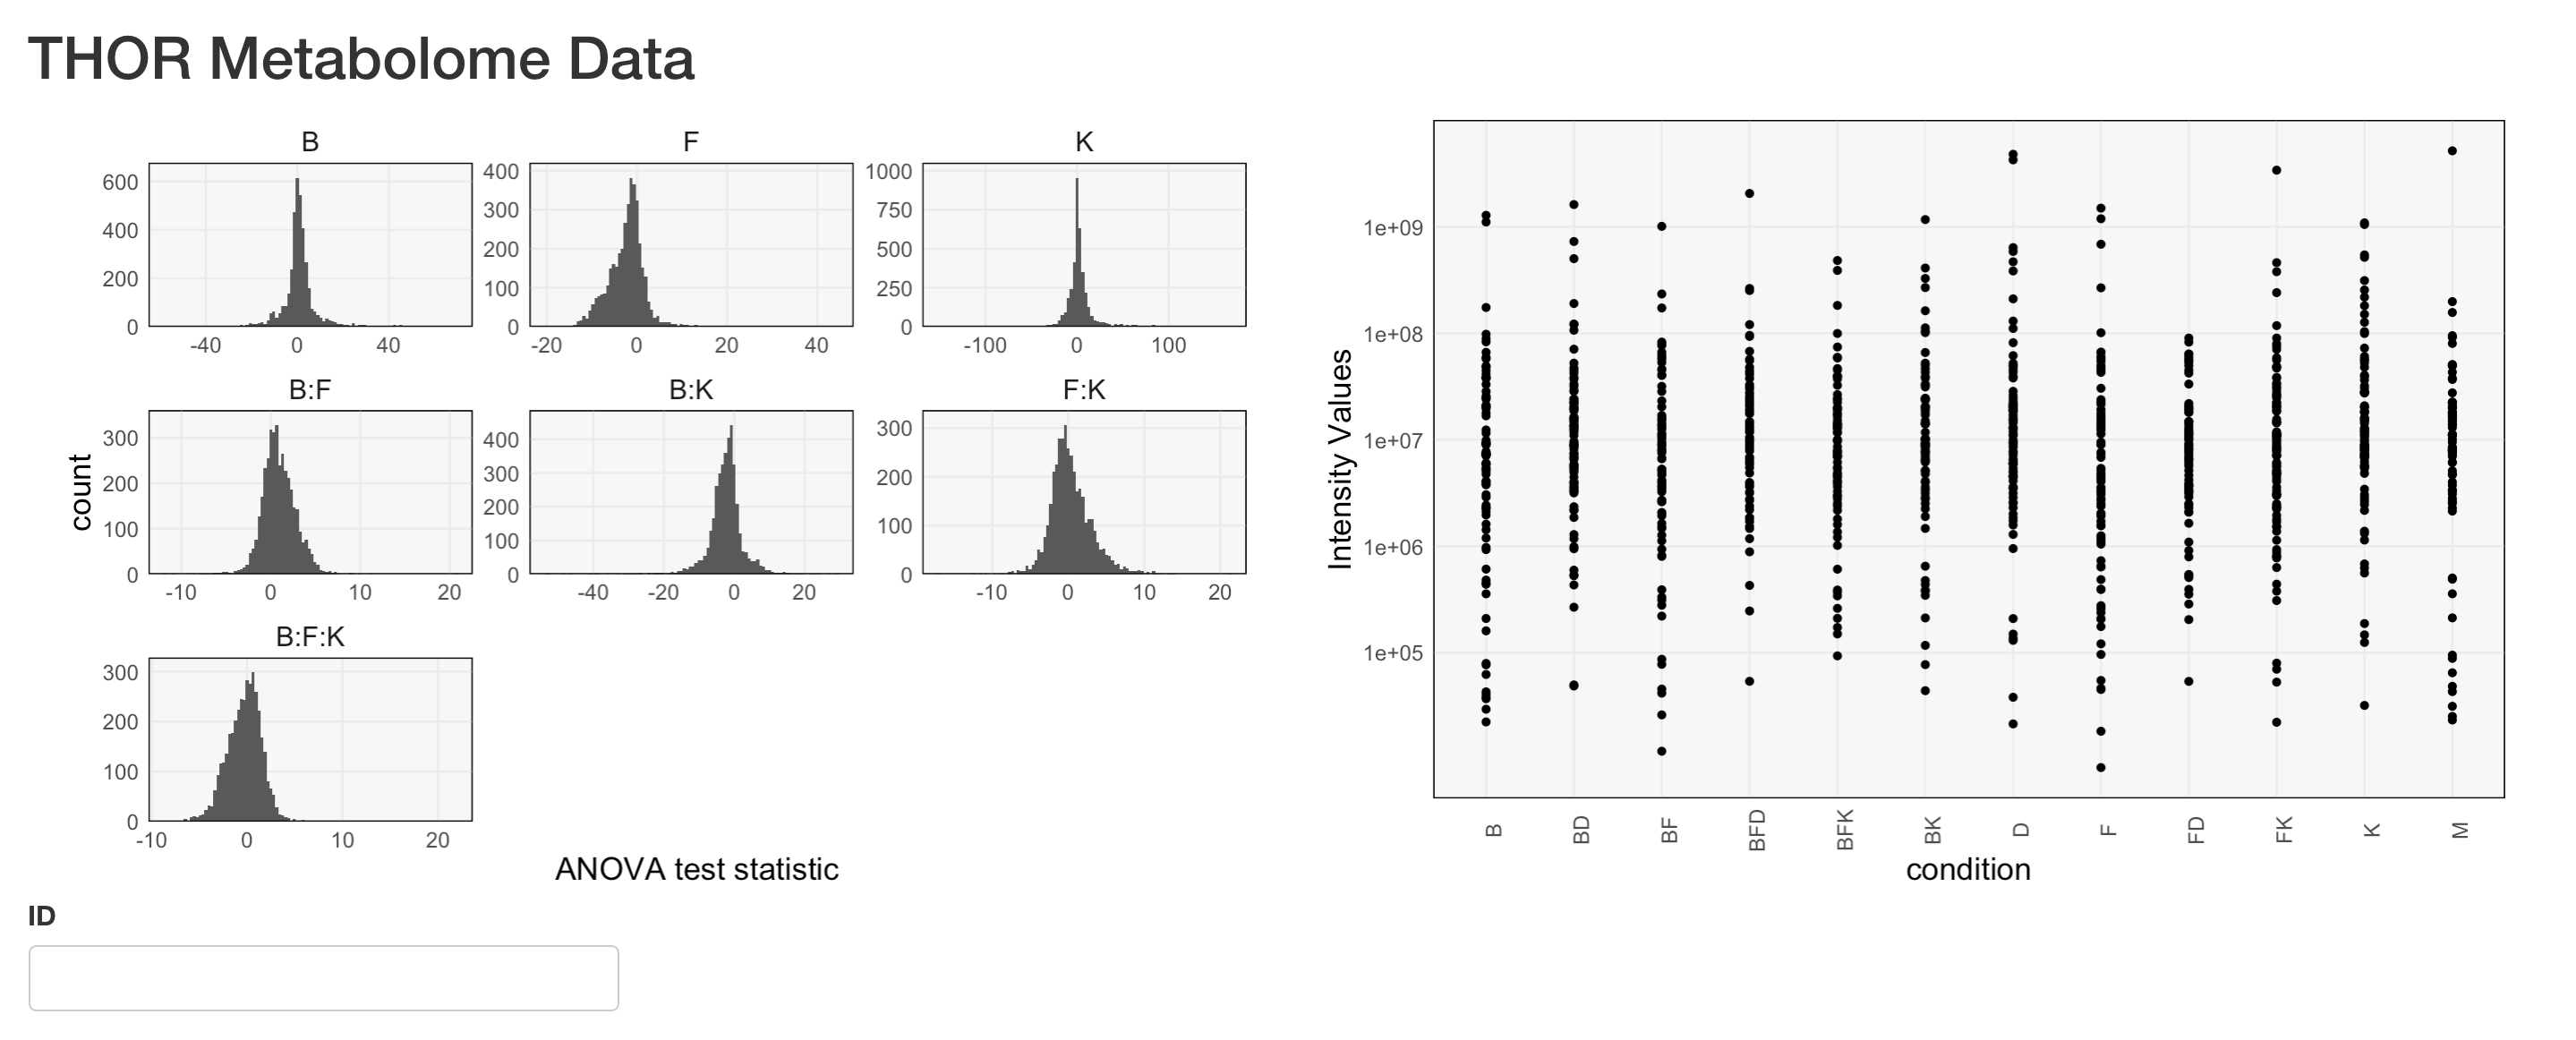
\includegraphics{/Users/tuyixing/Desktop/Course/research/before.png}
\caption{Example1.1}
\end{figure}

In the figure below, we brushed compounds with large, positive F
effects. The reflected negative effect compounds are in orange. In this
selection, the associated FK effects are mostly positive and the
associated BFK effects are mostly negative (compare the orange bulk
within this panel with 0). A possible explanation is that these
selected, orange compounds are consumed by F, which is why they decrease
in the presence of F. The positive FK effects suggest that these
compounds are not being consumed as rapidly when K is present. This is
consistent with our understanding of the system\ldots{}

But when all three are present, the compound is less abundant again, it
is an evidence for B protecting F.

In this way, MTBrush has helped clarify the mechanisms that underlie
emergent phenomena that have

\begin{figure}
\centering
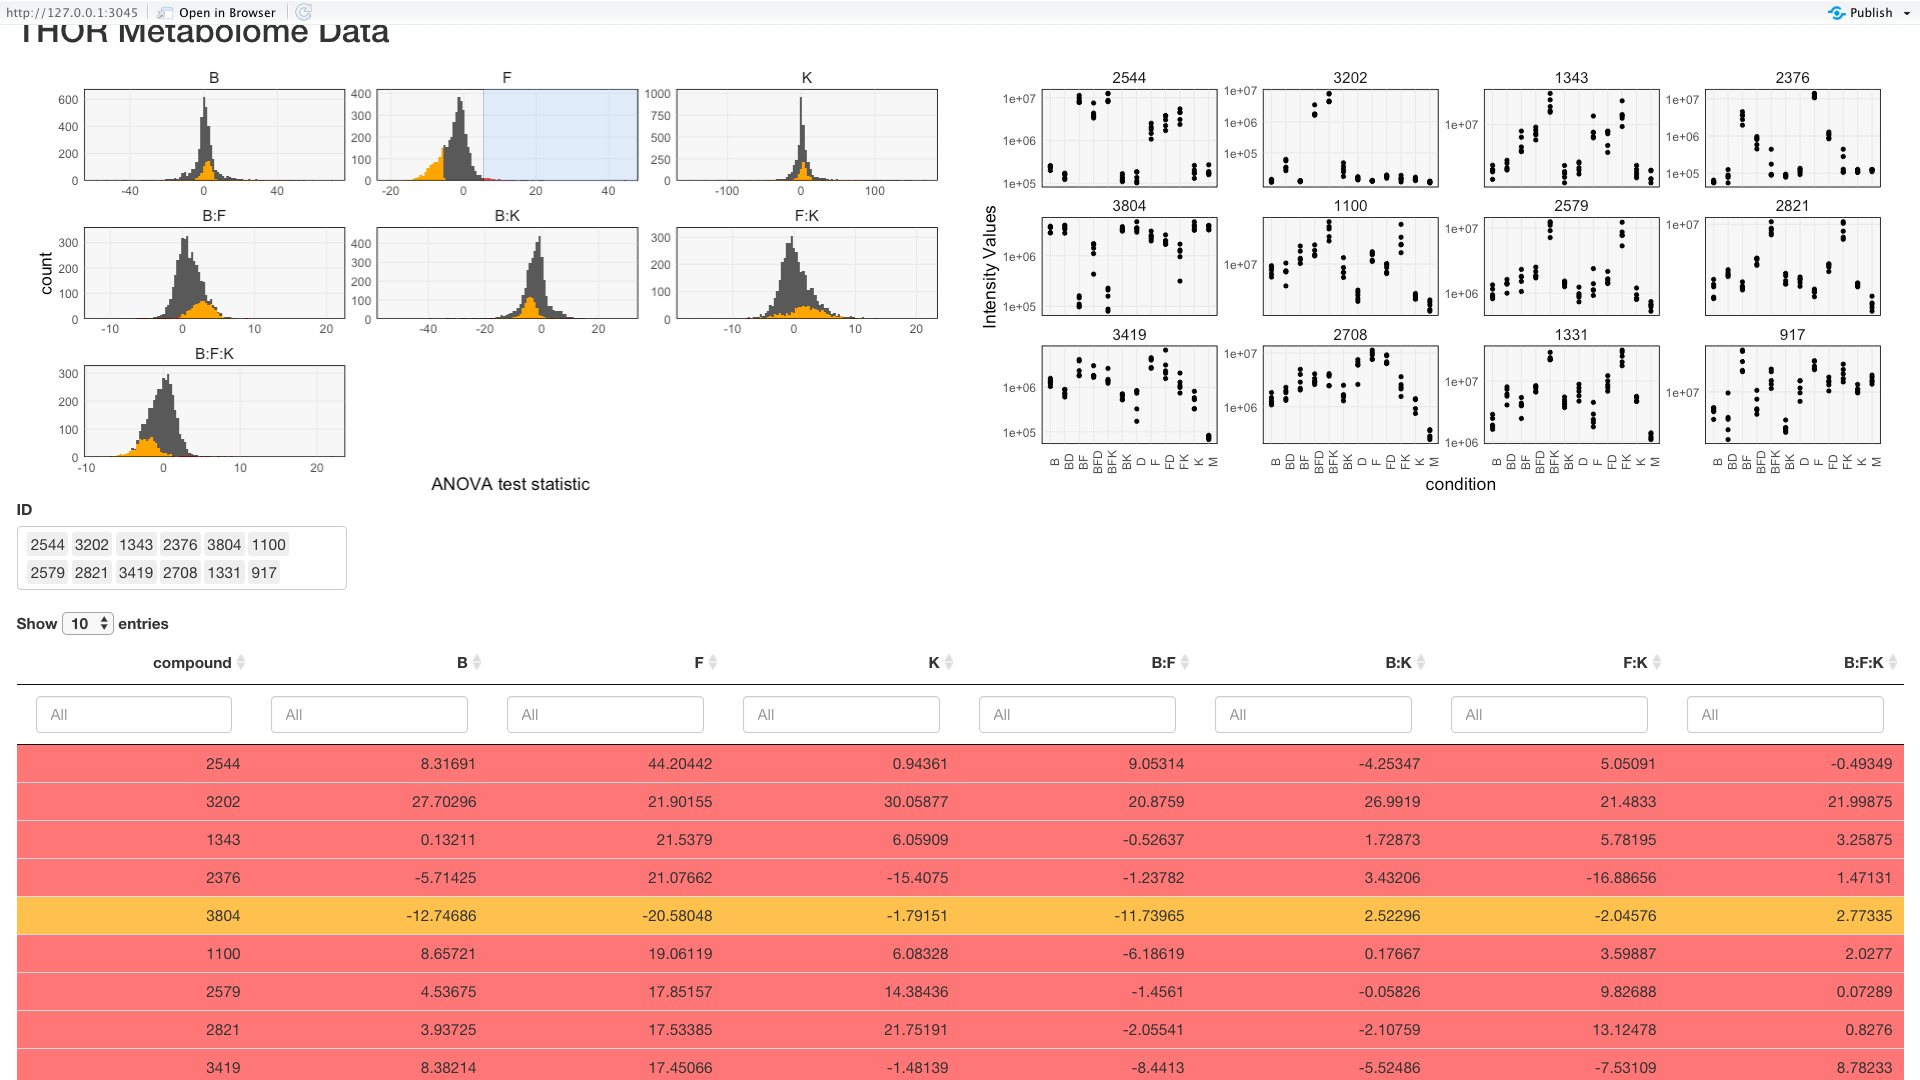
\includegraphics{/Users/tuyixing/Desktop/Course/research/Thor_example.png}
\caption{Example1.2}
\end{figure}

\hypertarget{navigating-california-home-prices}{%
\subsection{Navigating California home
prices}\label{navigating-california-home-prices}}

Our next example uses \texttt{MTBrush} to support exploration of the
California Housing Price dataset \cite{give citation}. This dataset
includes prices of 20,640 homes, together with features of the homes and
their neighborhoods, including the number of rooms and neighborhood's
median income, for example. These data are often used to evaluate
supervised learning methods. Our focus instead is to visualize how the
conditions of a home and neighborhood relate to observed prices, and how
these effects vary geographically.

Specifically, to understand how the influence of home and neighborhood
features are modulated by geographic location, we partition the dataset
into geographically disjoint sets and fit a linear model within each.
The coefficients from these models can be plotted as histograms and
brushed to identify features that are important in some locations but
not others. Since some locations have many more houses than others,
partitioning the data with a simple geographic grid would result in
highly imbalanced sample sizes across the ensemble. For areas with
limited number of houses, the results would not be comparable to those
in areas with larger sample sizes. To address this, we first apply
K-means to the geographic coordinates of the observed homes, resulting
in 2064 clusters with more balanced sample sizes.

Figure \ref{fig:homestart} shows the distribution of variable features
before any user interactions. From this overview, we notice that the
home prices are inversely related to the population density. In Figure
\ref{fig:homebrush}, we brushed to highlight those houses with positive
households effects. We find that the corresponding households and median
income interaction effects are negative, suggesting that median income
restrains the positive effects of households. Specifically, an increase
in the median income of a neighborhood has a smaller effect on average
home price when the number of households in that neighborhood is large.
When the population variable is also added, the three-way interaction
term seems to have a positive effects again.

For this dataset, it is typical to fit a single nonlinear model use it
to make predictions for house price. Interpreting the result of this fit
can be challenging, however. In contrast, by interacting with a full
ensemble of simple models, we can easily compare geographic variation in
effects, using individual panels to observe characteristics of
individual homes in each area.

\begin{figure}
\centering
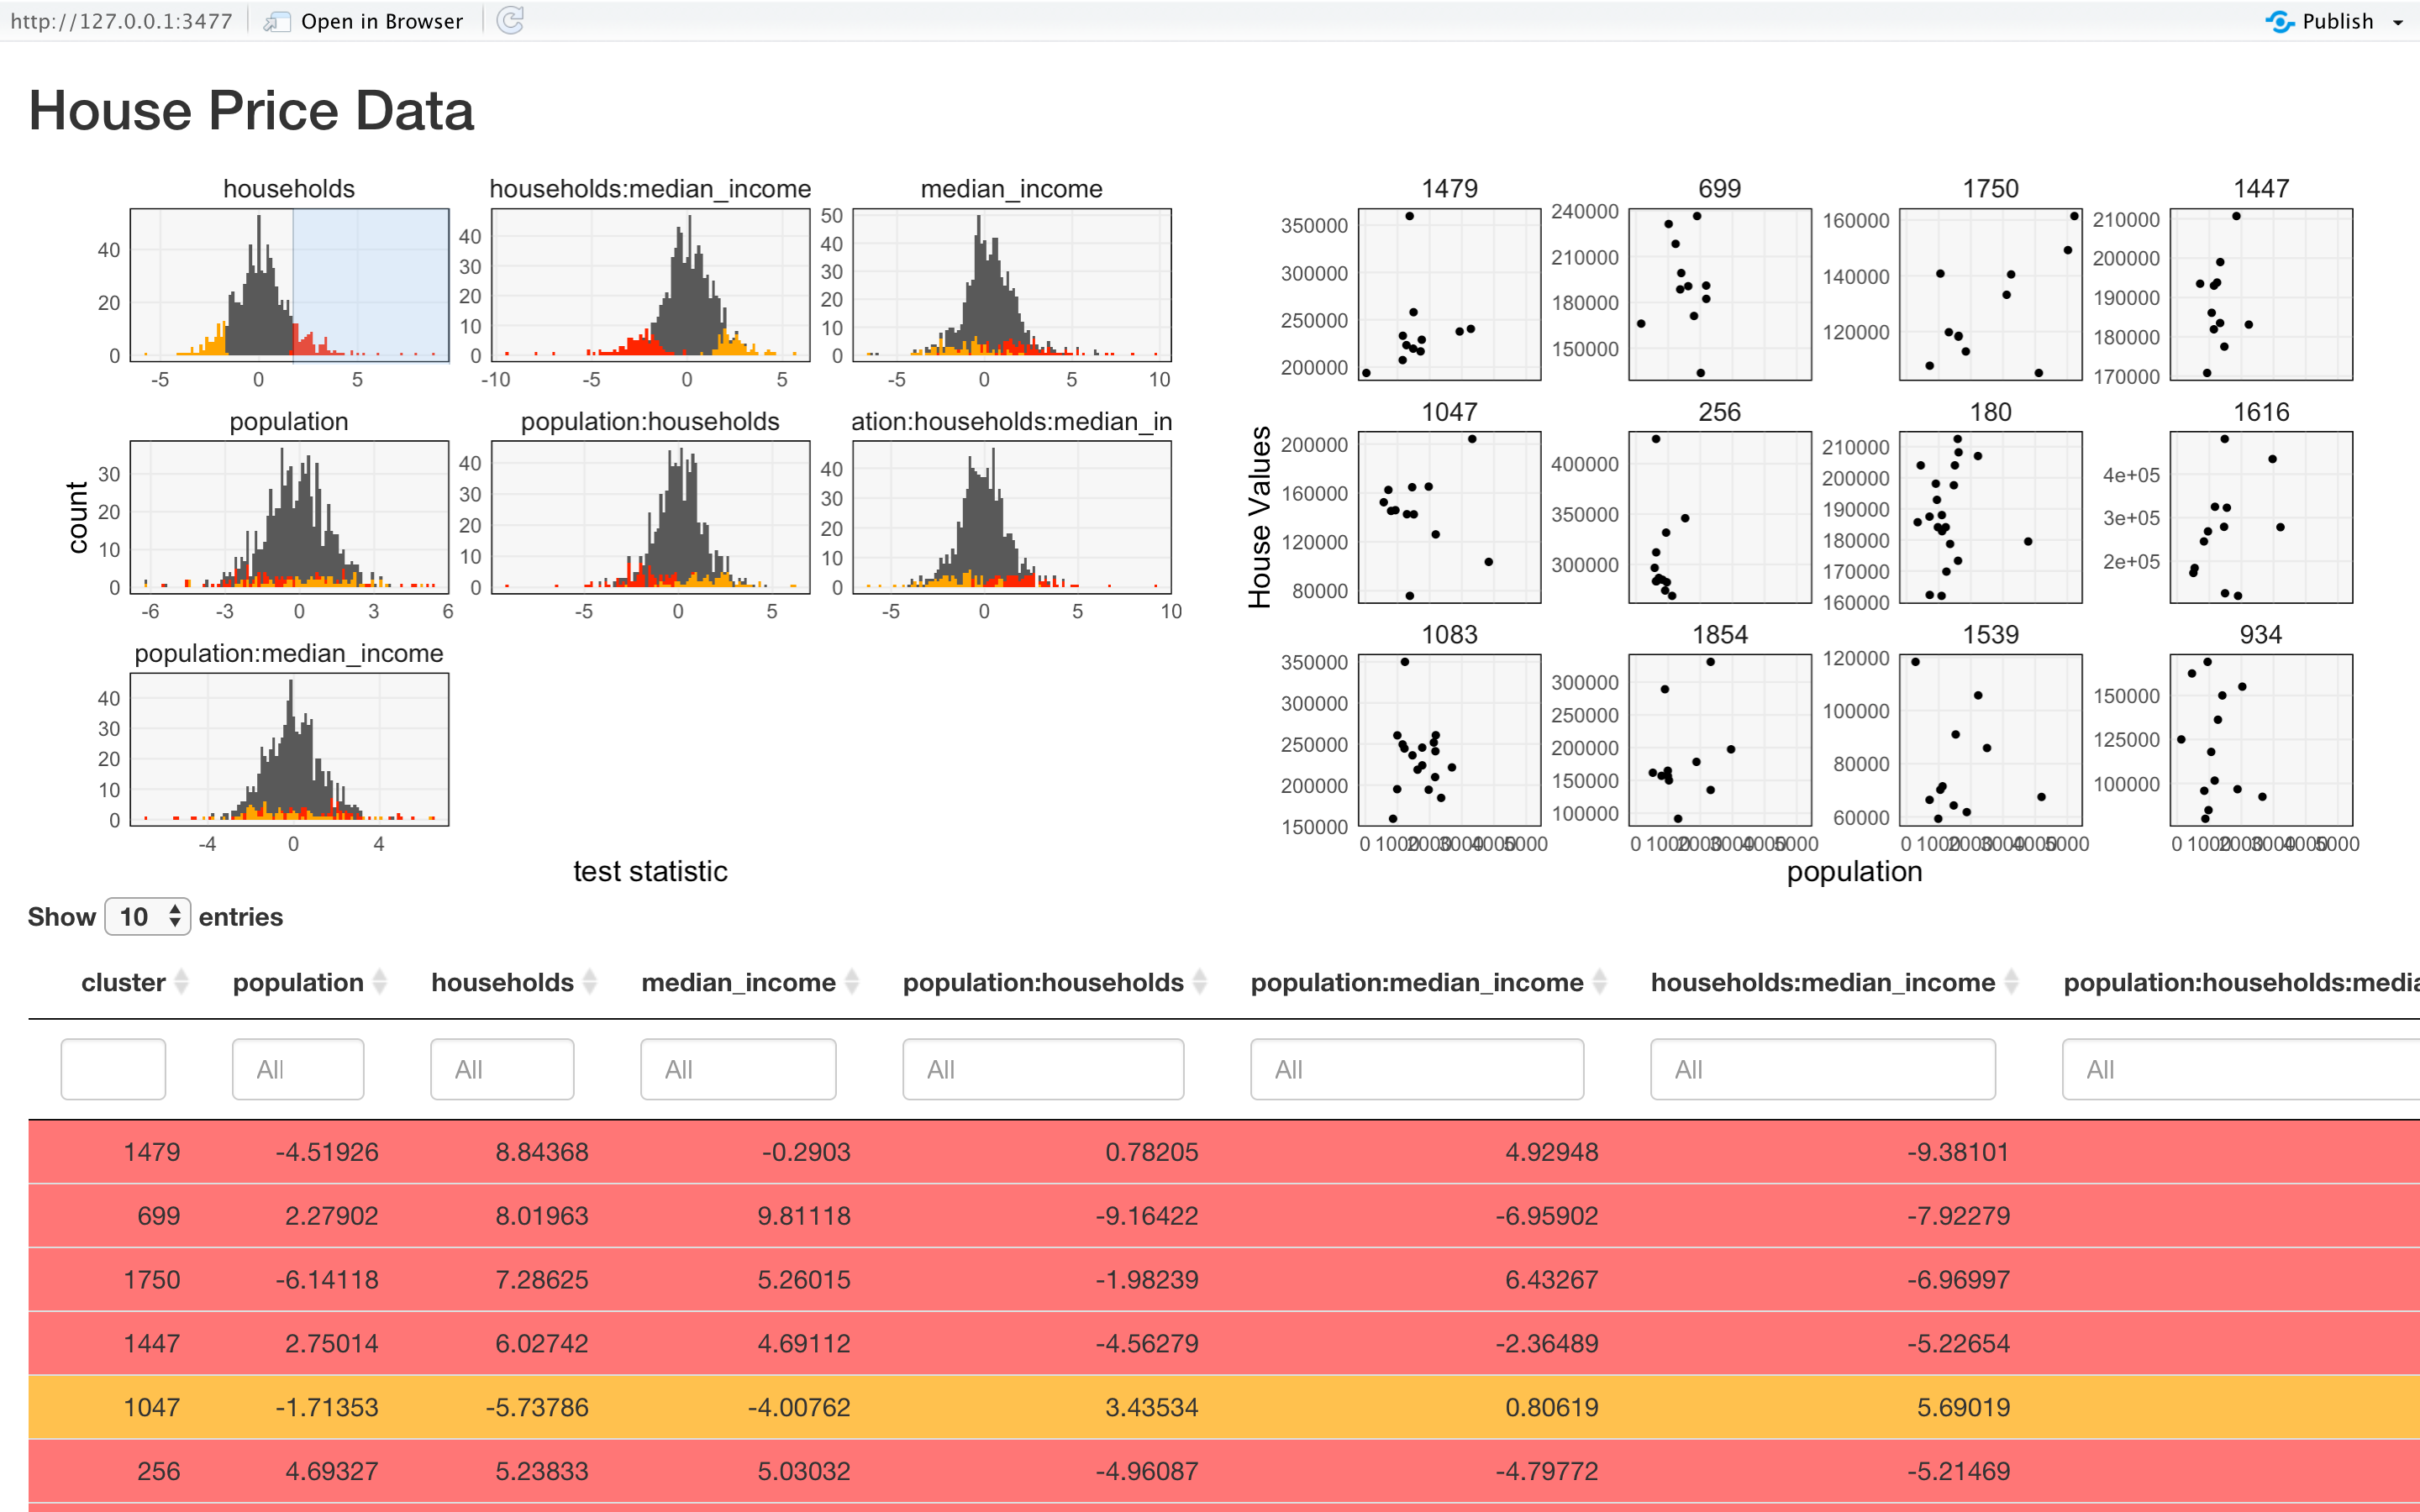
\includegraphics{/Users/tuyixing/Desktop/Course/research/example2.png}
\caption{Example2}
\end{figure}

\hypertarget{discussion}{%
\section{Discussion}\label{discussion}}

This package help to perform a multiple hypothesis testing for similar
samples in a large number of groups. After clean the data into the type
of input data on the pipeline, given a model, we can easily apply the
model to all the groups and visualize test statistics. Then by brushing
through linked diagrams, we can interpret the data in a more intuitive
and efficient way.

However, currently we give users the freedom to use their own model and
believe that the model is valid, so in the future work we will put some
effort on checking the correctness and effectiveness of the model like
implementing the multiple hypothesis testing outputs. we will include a
more complete process of hypothesis testing including null and
alternative hypothesis. We will pay attention to the p-value and avoid
rejecting the null hypothesis due to the tolerance of significant level
when dealing with a bunch of test statistics. In the future, we will
consider adding multiple brushes to the panel so that we will get more
information from plots and it will be easier to compare. Lastly, we may
add method to deal with data sets contains the mixing of binary and
non-binary variables, since this package only apply to binary or
non-binary data type.

Download the MTBrush package through:
remotes::install\_github(``YixingTT/MTBrush/MTBrush'')

\hypertarget{bibliography}{%
\section{Bibliography}\label{bibliography}}

\end{document}
